\section{软件设计概述}
\label{sec:introduction}

\begin{frame}
  \begin{center}
    \Huge{\textcolor{red}{软件设计概述}}
  \end{center}
\end{frame}

\subsection{设计初衷}

\begin{frame}{设计目标}
  \begin{figure}
    \centering
    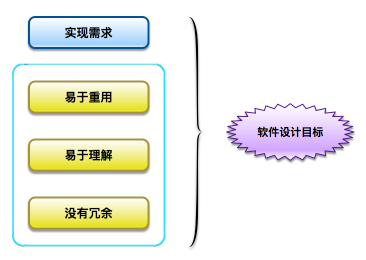
\includegraphics[width=0.7\textwidth]{design-goal.png}
  \end{figure}
\end{frame}

\begin{frame}{易于重用}
  \begin{figure}
    \centering
    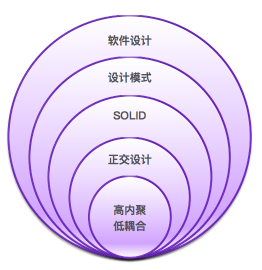
\includegraphics[width=0.5\textwidth]{methodology.png}
  \end{figure}
\end{frame}

\begin{frame}{易于理解}
  \begin{columns} 
  \begin{column}{0.3\textwidth}
  \begin{enumerate}
    \item \alert{Clean Code}
    \item \alert{Idioms}
    \item \alert{Patterns}
  \end{enumerate}
  \end{column}  

  \begin{column}{0.7\textwidth}
  \begin{figure}
    \centering
    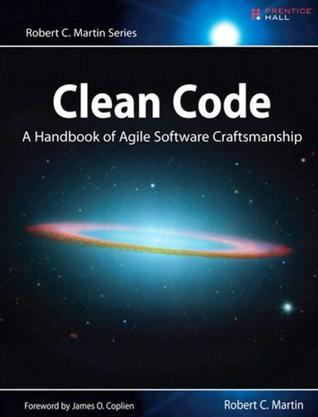
\includegraphics[width=0.5\textwidth]{clean-code.jpg}
  \end{figure}
  \end{column}
  \end{columns}   
\end{frame}

\begin{frame}{没有冗余}
  \begin{enumerate}
    \item \alert{YAGNI}: You Ain't Gonna Need It
    \item \alert{KISS}: Keep it Simple, Stupid
  \end{enumerate}
\end{frame}

\subsection{正交设计}

\begin{frame}{模块化设计}
  \begin{figure}
    \centering
    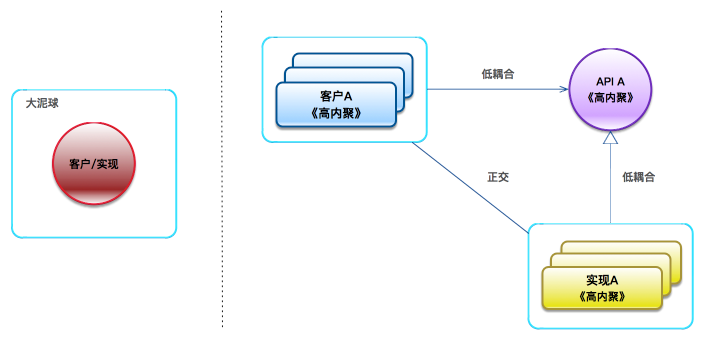
\includegraphics[width=1.0\textwidth]{module-design.png}
  \end{figure}
\end{frame}

\begin{frame}{高内聚低耦合}
\begin{columns} 
  \begin{column}{0.5\textwidth}
  \begin{figure}
    \centering
    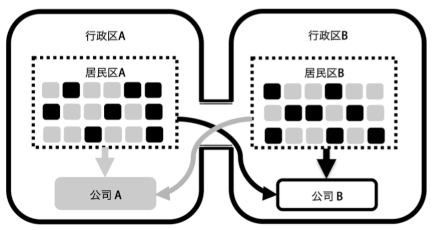
\includegraphics[width=0.9\textwidth]{low-cohesion-hign-coupling.png}
  \end{figure}
  \end{column}
  
  \begin{column}{0.5\textwidth}
  \begin{figure}
    \centering
    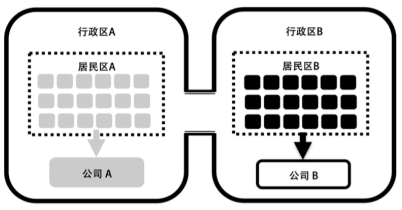
\includegraphics[width=0.9\textwidth]{high-cohesion-low-coupling.png}
  \end{figure}
  \end{column}
  \end{columns}  
\end{frame}

\begin{frame}{正交设计}
  \begin{figure}
    \centering
    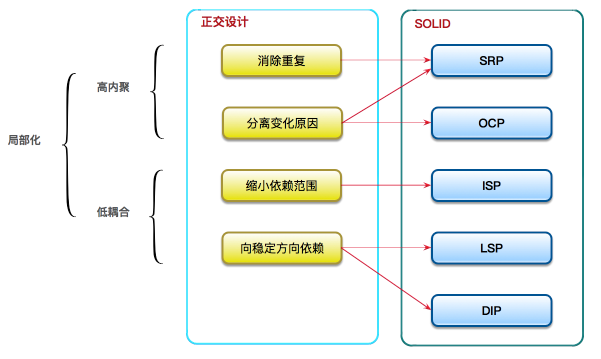
\includegraphics[width=0.9\textwidth]{orthogonal-design.png}
  \end{figure}
\end{frame}

\begin{frame}{拥抱变化}
  \begin{block}{应对变化} 
    \begin{enumerate}
    \item \alert{一个变化导致多处散弹修改}:消除重复
    \item \alert{多个变化导致一处频繁修改}:分离变化
    \end{enumerate}
  \end{block}

  \begin{block}{变化发生时,消除不必要的修改} 
    \begin{enumerate}
    \item \alert{不依赖不必要的依赖}:缩小依赖范围
    \item \alert{不依赖不稳定的依赖}:向着稳定的方向依赖
    \end{enumerate}
  \end{block}
\end{frame}
